\documentclass[12pt]{article}
\usepackage{minted}
\usepackage{graphicx}
\usepackage[margin=0.25in]{geometry}

\begin{document} 
	\noindent
	Dan Jandel C. De Ramos\\
	BSCpE 2-1\\
	Made with \LaTeX \\
	GitHub repo link: https://github.com/Joatmon-21/De-Ramos-CMPE201\\
	\\
	Activity 1 (Same as Sample)\\
	Source Code:
	\begin{minted}[tabsize=5]{java}         
/*
* Written by: Dan Jandel C. De Ramos
* Polytechnic University of the Philippines Biñan
* Bachelor of Science in Computer Engineering 2-1
*/
		
public class Activity_1_SAS{
	public static void main(String[]args){         
				
		//The data stored here are for the sake of examples only and are not 100% accurate        
		String name = "Juan S. Dela Cruz";        
		char gender = 'm';        
		boolean maritalStatus = true;
		byte numberOfChildren = 8;
		short birthYear = 1945;
		int salary = 88000;  
		long netAsset = 8234567890L;
		double weight = 88.88;
		float gpa = 3.88f;
				
		System.out.println("Name is : " + name);
		System.out.println("Gender is : " + gender);
		System.out.println("Is married is : " + maritalStatus);
		System.out.println("Number of Children is : " + numberOfChildren);
		System.out.println("Year of birth is : " + birthYear);
		System.out.println("Salary is : " + salary);
		System.out.println("Net Asset is : " + netAsset);
		System.out.println("Weight is : " + weight);
		System.out.println("GPA is : " + gpa);       
	}
}
	\end{minted}
	\clearpage
	\noindent
	Output:\\
	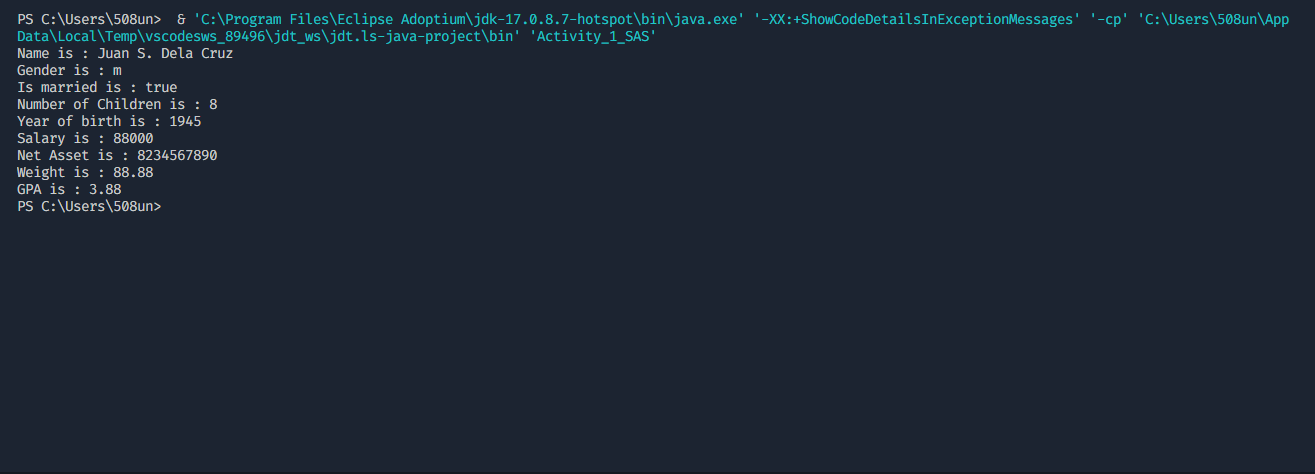
\includegraphics[width=\textwidth]{output1SAS}
	\clearpage
	\noindent
	Activity 1\\
	Source Code:
	\begin{minted}[tabsize=5]{java}         
/*
* Written by: Dan Jandel C. De Ramos
* Polytechnic University of the Philippines Biñan
* Bachelor of Science in Computer Engineering 2-1
*/
		
public class Activity_1{
	public static void main(String[]args){         
				
		//The data stored here are for the sake of examples only and are not 100% accurate        
		String name_1 = "Dan Jandel C. De Ramos";        
		char gender = 'M';
		char pesoSign = '\u20B1';
		boolean maritalStatus = false;
		byte numberOfChildren = 0;
		short birthYear = 2003;
		int salary = 65536;  
		long netAsset = 89414685416L;
		double weight = 69.42;
		float gpa = 1.88f;
		
		System.out.println();
		
		System.out.println(" \u2022 Activity # 1 \u2022 \n");
		System.out.println("Name: " + name_1);
		System.out.println("Gender: " + gender);
		System.out.println("Married: " + maritalStatus);
		System.out.println("Number of Children: " + numberOfChildren);
		System.out.println("Year of birth: " + birthYear);
		System.out.println("Salary: " + pesoSign + " " + salary);
		System.out.println("Net Asset: " + pesoSign + " " + netAsset);
		System.out.println("Weight: " + weight + "kg");
		System.out.println("GPA: " + gpa);       
				
		System.out.println();        
	}
}
	\end{minted}
	\clearpage
	\noindent
	Output:\\
	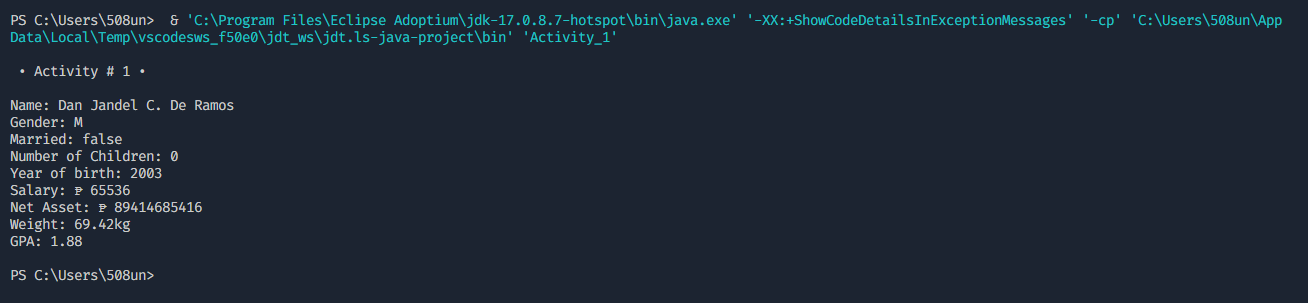
\includegraphics[width=\textwidth]{output1}
	\clearpage
	\noindent
	Activity 2 using next()\\
	Source Code:
	\begin{minted}[tabsize=5]{java}         
/*
* Written by: Dan Jandel C. De Ramos
* Polytechnic University of the Philippines Biñan
* Bachelor of Science in Computer Engineering 2-1
*/

import java.util.Scanner;

public class Activity_2_n{
	public static void main(String[]args){
		
		Scanner favoriteFruitScanner = new Scanner(System.in);
		String favoriteFruit;
		
		Scanner favoriteColorScanner = new Scanner(System.in);
		String favoriteColor;
		
		System.out.println();
		
		System.out.println("\u2022 Activity 2 using next() \u2022");
		
		System.out.println();
		
		System.out.println("What is your favorite fruit?");
		favoriteFruit = favoriteFruitScanner.next();    
		
		System.out.println();
		
		System.out.println("What is your favorite color?");
		favoriteColor = favoriteColorScanner.next();
		
		favoriteFruitScanner.close();
		favoriteColorScanner.close();
		
		System.out.println();        
		
		System.out.println("I wonder what a " + favoriteColor + " " + favoriteFruit + " would taste like");
		
		System.out.println();
		
	}
}
	\end{minted}
	\clearpage
	\noindent
	Output:\\
	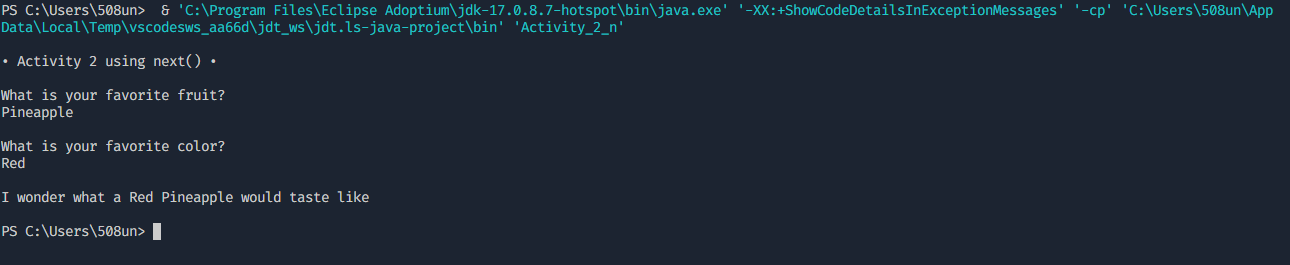
\includegraphics[width=\textwidth]{output2n}	
	\clearpage
	\noindent
	Activity 2 using nextLine()\\
	Source Code:
	\begin{minted}[tabsize=5]{java}         
/*
* Written by: Dan Jandel C. De Ramos
* Polytechnic University of the Philippines Biñan
* Bachelor of Science in Computer Engineering 2-1
*/
		
import java.util.Scanner;
import java.util.InputMismatchException;
		
public class Activity_2{
	public static void main(String[]args){
				
		Scanner input = new Scanner(System.in);
				
		String name;
		String location;
		short age = 0;
				
		System.out.println();
		
		System.out.println("\u2022 Activity # 2 \u2022 \n");
		System.out.println("What is your name? ");
		name = input.nextLine();
		System.out.println("\nWhat is your age in years? ");        
		while(age==0){            
			try {
			age = input.nextShort();
			} catch (java.util.InputMismatchException e) {            
				System.out.print("\n!!! You have entered an invalid value.");
				System.out.println("Please use whole numbers only !!!");  
				System.out.println("What is your age in years?");
				input.next();          
			}
		}
		
		input.nextLine();
		System.out.println("\nWhere do you live?");
		location = input.nextLine();
		input.close();
		System.out.println("\nYour name is " + name);
		System.out.println("You are " + age + " years old");
		System.out.println("You live in " + location);
	
		System.out.println();
	}
}
	\end{minted}
	\clearpage
	\noindent
	Output:\\
	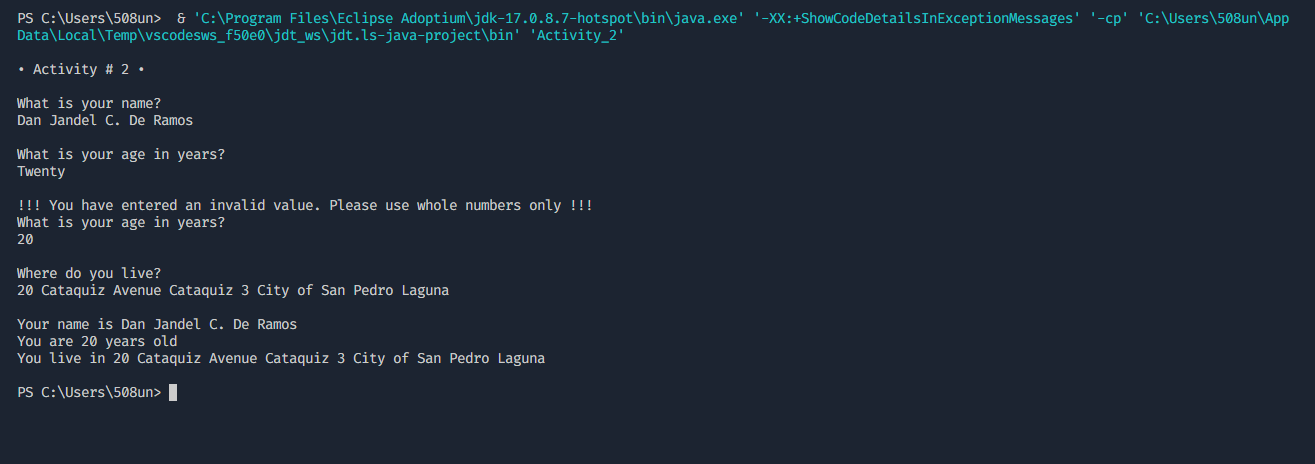
\includegraphics[width=\textwidth]{output2nL}
\end{document}